\documentclass[10pt,a4paper]{article}
\usepackage[margin=0.5in]{geometry}
\usepackage{enumitem}
\usepackage{amsmath}
\usepackage{multicol}
\usepackage{graphicx}

\begin{document}
\pagestyle{empty}

\begin{center}
    \textbf{FEDERAL UNIVERSITY OF RIO GRANDE DO SUL}\\
    \textbf{INSTITUTE OF INFORMATICS}\\
    \vspace{3.2in}
    CMOS DEVICE ANALYSIS\\
    \vfill
    \textbf{PORTO ALEGRE}
\end{center}

\newpage

\begin{multicols}{2}
    \noindent\textbf{NMOS ANALYSIS}\\
    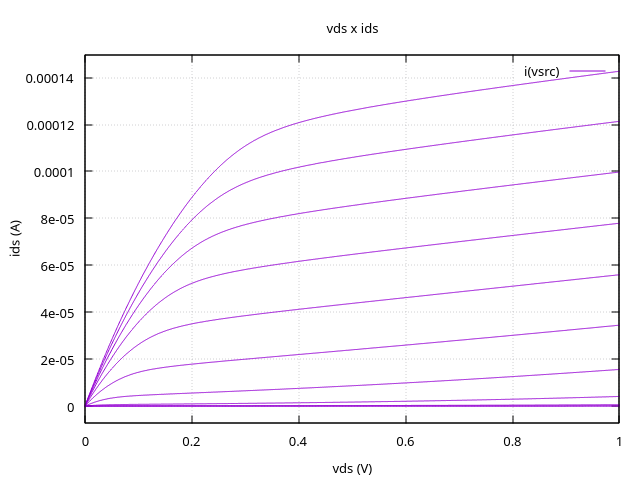
\includegraphics[width=0.5\textwidth]{vdsnmos} 
    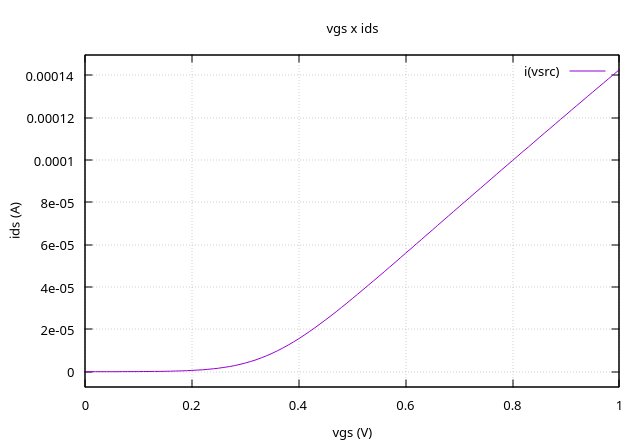
\includegraphics[width=0.5\textwidth]{vgsnmos} 
    \noindent\textbf{PMOS ANALYSIS}\\
    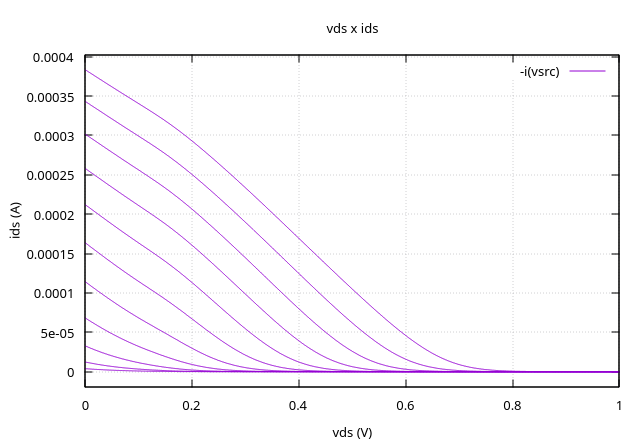
\includegraphics[width=0.5\textwidth]{vdspmos} 
    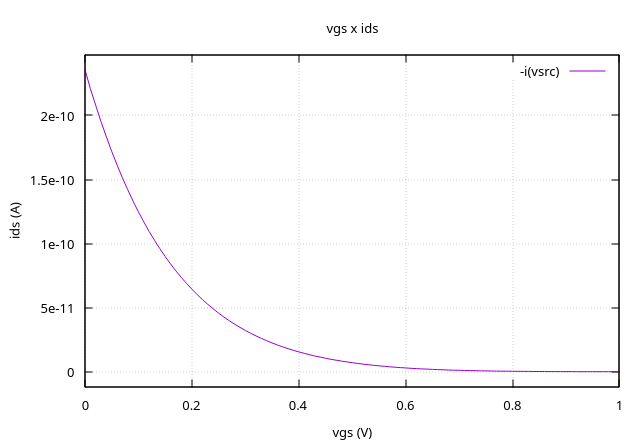
\includegraphics[width=0.5\textwidth]{vgspmos} 
\end{multicols}

\noindent\textbf{OBSERVATIONS}\\
\noindent The maximum current conducted by the NMOS transistor was six orders of magnitude ($10^6$) higher than that of the PMOS transistor. Furthermore, the NMOS starting current was slightly above zero, while the PMOS current dropped to actual zero at the end of its sweep -- a curious disparity. This difference at the voltage limits is currently unexplained, although simulation imprecision may be a factor. Ultimately, increasing the PMOS width ratio to compensate for its lower conductance proved insufficient, since a significant difference between the two models persists.

\end{document}
